\documentclass[titlepage, letterpaper]{article}
\usepackage[utf8]{inputenc}
\usepackage{fancyhdr} % fancy headers, of course!
\usepackage{amsmath} % what do you think?
\usepackage{amsthm} % theorems!
\usepackage{extramarks} % more cute things
\usepackage{enumitem} % i'm not sure...
\usepackage{multicol} % multicolumn...?
\usepackage{amssymb} % more symbols
\usepackage{MnSymbol} % moar symbols?
\usepackage{booktabs} % cool looking tables
\usepackage{tikz} %venn and shizzle
\usepackage{mathrsfs} %math script for calligraphic scripting, I GUESS
\usepackage{listings}
\usepackage{mathtools}
\usepackage{graphicx}
\usepackage{subcaption}
\usepackage{gensymb}
\usepackage{textcomp}
\usepackage[draft, author=, mode=singleuser]{fixme}


\topmargin=-0.45in
\evensidemargin=0in
\oddsidemargin=0in
\textwidth=6.4in
\textheight=9.0in
\headsep=0.25in

\fxusetheme{colorsig} % theme for fixme
\fxsetface{margin}{\ttfamily\tiny}

\title{
\vspace{1in}
\textbf{Tecnológico de Monterrey} \\
\vspace{0.5in}
\textmd{Robotics} \\
\large{\textit{Dr. Ernesto Rodríguez Leal}} \\
\vspace{0.5in}
\textsc{Kinematic Analysis of a 3-RSP parallel mechanism}\\
\author{00783957 -- Alicia del Río \\
\and 00952040 -- Cristina Aparicio \\
\and 00822833 -- Guillermo Sotelo \\
\and 00809576 -- Sergio Sedas \\
\and 01170065 -- Xavier Sánchez}
\date{\today}
}

\DeclareMathOperator{\cose}{\mathcal{C}}
\DeclareMathOperator{\sen}{\mathcal{S}}
\newcommand{\spacepls}{\vspace{5mm}}

\begin{document}
%\listoffixmes
\maketitle

\begin{abstract}
This paper presents a kinematic analysis of a 3-\underline{R}SP parallel mechanism.
The structure of the mechanism is formed by a fixed base and three identical legs of three links connected by a revolute, spherical and prismatic joints from base to top platform.
The paper includes forward and inverse position analysis, velocity and singularity analysis using screw theory, static and dynamic analysis, and the problems presented during the analysis phase for this particular configuration.
Results of motion simulation with SolidWorks are then compared with theoretical results obtained from Mathematica.
% \keywords{Parallel mechanism, RSP architecture, Forward kinematics, Inverse kinematics, Instantaneous screw axis, Jacobian matrix}
\end{abstract}


\section{Introduction}
\label{sec:intro}

A parallel mechanism consists of a series of links arranged in a closed kinematic chain connecting the base to the end-effector.
This type of configuration results in greater structural rigidity and accuracy than serial or open chain robots.
However, the drawback of this type of configuration is a smaller workspace due to link interference and greater complexity for analysis due to the closed kinematic loops of equations.
Nonetheless, parallel manipulators are the best alternative for applications requiring high load carrying capacity and precise positioning due to higher structural stiffness, reduced sensitivity to errors and built-in redundancy.
This paper focuses on the kinematics of a 3-\underline{R}SP mechanism with 3 degrees of freedom (DOF), where the R denotes a revolute joint which is actuated and fixed to the base, S denotes a spherical joint and P a prismatic joint connecting to the superior platform.

The paper is organized as follows:
Section~\ref{sec:geo} contains a description of the mechanism's geometry.
Forward and inverse position analysis is presented in Section~\ref{sec:analysis} and~\ref{sec:inverse}.
Sections~\ref{sec:mobility}, \ref{sec:velocity} and \ref{sec:singular} include the velocity and singularity analysis using screw theory.
Static and dynamic analysis is described in Sections \ref{sec:static} and \ref{sec:dynamic}.
Additionally, some details about the motion study and the building of the prototype are presented in Sections~\ref{sec:motion_study} and \ref{sec:prototype}.
Section~\ref{sec:problems} details problems presented during the analysis phase for this particular configuration.
Finally, Section~\ref{sec:conc} concludes the study.

It is important to note that we use a special notation for some trigonometric functions: sines are represented with $\sen$ and cosines with $\cose$.

\section{Geometry}
\label{sec:geo}

The geometry of the 3-\underline{R}SP consists of a fixed base connected by three identical legs to a movable platform.
Each leg is comprised of three links where the first link is connected to the base by a revolute joint.
The second link is then connected to the first link by a spherical joint.
The third link is the platform connected to the second link by a prismatic joint.
The resulting geometry is the chain of RSP joints of the mechanism.
The actuated joints are the revolute joints (hence, the underlining in the text).
Fig.~\ref{fig:3dmodel} shows the 3D model of the mechanism.

\begin{figure}[htbp]
    \centering
    \includegraphics[width=0.75\textwidth]{fig_3dmodel}
    \caption{The 3-RSP mechanism 3D model}
    \label{fig:3dmodel}
\end{figure}

A schematic drawing of leg $i$ ($i = 1, 2, 3$) is shown in Fig.~\ref{fig:schema}.
The subscripts $i_j$ denote joint $j ( j = 1, 2, 3, 4, 5)$ in leg $i$.
The spherical joint is represented as three revolute joints:
one for each orthogonally intersecting axis of movement ($x, y, z$).
The revolute joints are equally distributed on the base and the locations are defined by vector $a_i$, going from the center of the base to the center of revolute joint $i$.
The spherical and prismatic joints are coincident at some point. The vector going from the revolute joint to this coincident point is denoted as $d_i$.
The axes of the prismatic joints intersect at the center of the platform.
The vector going from the center of the platform to the center of the sphere is the vector $b_i$.
Vector $p$ defines the position from the center of the base to the center of the platform.
The notation used is quite similar as the one used in~\cite{Rodriguez-Leal11}.

\begin{figure}[htbp]
    \centering
    \begin{subfigure}[b]{0.45\textwidth}
        \includegraphics[width=\linewidth]{fig_schema_a}
    \end{subfigure}
    \begin{subfigure}[b]{0.45\textwidth}
        \includegraphics[width=\linewidth]{fig_schema_b}
    \end{subfigure}
    \caption{Schematic drawing for the $i$-th leg.}
    \label{fig:schema}
\end{figure}

\section{Analysis}
\label{sec:analysis}

Since the mechanism is comprised of three identical legs, the position and orientation of the platform can be obtained from the study of only one of them. A position analysis of the platform is performed and geometrical constraints applied to the closed loop equation.

The closed loop equation for leg $i$ can be written as

\begin{equation}
\label{eq:closed_loop}
    p + b_i = a_i + d_i
\end{equation}

where

\begin{equation}
    \label{eq:p}
    \mathbf{p} = [p_x, p_y, p_z]^T
\end{equation}

\begin{equation}
    \label{eq:a}
    \mathbf{a}_i = \mathbf{R}(Z,\psi_i) \cdot [a_i,0,0]^T
\end{equation}

\begin{equation}
    \label{eq:b}
    \mathbf{b}_i = \mathbf{R}(Z,\chi_i) \cdot \mathbf{R}(Z,\gamma_i) \cdot \mathbf{R}(T,\beta_i) \cdot [0, b_i, 0]^T
\end{equation}

\begin{equation}
    \label{eq:d}
    \mathbf{d}_i = \mathbf{R}(Z,\psi_i) \cdot \mathbf{R}(Z',\phi) \cdot \mathbf{R}(X'',\theta_{i}) \cdot [0, d_i, 0]^T
\end{equation}

The rotation matrices in Eq.~\ref{eq:a}, \ref{eq:b} and \ref{eq:d} are

\begin{equation}
    \label{eq:rot_Zpsi}
    \mathbf{R}(Z,\psi_i) =
    \begin{bmatrix}
        \cose\psi_i & -\sen\psi_i & 0 \\
        \sen\psi_i & \cose\psi_i & 0 \\
        0 & 0 & 1
    \end{bmatrix}
\end{equation}

\begin{equation}
    \label{eq:rot_Zphi}
    \mathbf{R}(Z,\phi_i) =
    \begin{bmatrix}
        \cose\phi_i & -\sen\phi_i & 0 \\
        \sen\phi_i & \cose\phi_i & 0 \\
        0 & 0 & 1
    \end{bmatrix}
\end{equation}

\begin{equation}
    \label{eq:rot_Xtheta}
    \mathbf{R}(X,\theta_i) =
    \begin{bmatrix}
        1 & 0 & 0 \\
        0 & \cose\theta_{i} & -\sen\theta_{i} \\
        0 & \sen\theta_{i} & \cose\theta_{i}
    \end{bmatrix}
\end{equation}

\begin{equation}
    \label{eq:rot_Zchi}
    \mathbf{R}(Z,\chi_i) =
    \begin{bmatrix}
    \cose\chi_i & -\sen\chi_i & 0 \\
    \sen\chi_i & \cose\chi_i & 0 \\
    0 & 0 & 1
    \end{bmatrix}
\end{equation}

\begin{equation}
    \label{eq:rot_Xalpha}
    \mathbf{R}(X,\alpha) = 
    \begin{bmatrix}
    1 & 0 & 0 \\
    0 & \cose\alpha & -\sen \alpha \\
    0 & \sen\alpha & Cos \alpha
    \end{bmatrix}
\end{equation}

\begin{equation}
    \label{eq:rot_Ybeta}
    \mathbf{R}(Y,\beta) =
    \begin{bmatrix}
        \cose\beta & 0 & \sen\beta \\
        0 & 1 & 0 \\
        -\sen\beta & 0 &\cose\beta
    \end{bmatrix}
\end{equation}

\begin{equation}
    \label{eq:rot_Xgamma}
    \mathbf{R}(Z,\gamma) =
    \begin{bmatrix}
        \cose\gamma & -\sen\gamma & 0 \\
        \sen\gamma & \cose\gamma & 0 \\
        0 & 0 & 1
    \end{bmatrix}
\end{equation}
Additionally, the rotation matrix for the orientation of the platform is the following:

\begin{equation}
\label{eq:RM_matrix}
\begin{bmatrix}
 \cose \beta  \cose \gamma  & \cose \gamma  \sen \alpha  \sen \beta -\cose \alpha  \sen \gamma  & \cose \alpha  \cose \gamma  \sen \beta +\sen \alpha  \sen \gamma  \\
 \cose \beta  \sen \gamma  & \cose \alpha  \cose \gamma +\sen \alpha  \sen \beta  \sen \gamma  & \cose \alpha  \sen \beta  \sen \gamma -\cose \gamma  \sen \alpha  \\
 -\sen \beta  & \cose \beta  \sen \alpha  & \cose \alpha  \cose \beta  \\
\end{bmatrix}
\end{equation}

Substituting and performing the matrix multiplication gives

\begin{equation}
    \label{eq:a_substitute}
    \mathbf{a}_i =
    \begin{bmatrix}
    a_i \cose \psi_i \\
    a_i \sen \psi_i \\
    0
    \end{bmatrix}
\end{equation}

\begin{equation}
    \label{eq:b_substitute}
    \mathbf{b}_i =
    \begin{bmatrix}
    (\cose \beta \cose \gamma \cose \chi_i + (\cose \gamma \sen \alpha \sen \beta - \cose \alpha \sen \gamma)\sen \chi_i) b_i \\
    (\cose \beta \cose \chi_i \sen \gamma + (\cose \alpha \cose \gamma \ \sen \alpha \sen \beta \sen \gamma)\sen \chi_i) b_i \\
    (-\cose \chi_i \sen \beta + \cose \beta \sen \alpha \sen \chi_i) b_i
    \end{bmatrix}
\end{equation}

\begin{equation}
    \label{eq:d_substitute}
    \mathbf{d}_i =
    \begin{bmatrix}
    -d \cose \theta_i \cose \psi_i \\
    -d \cose \theta_i \sen \psi_i \\
    d \sen \theta_i
    \end{bmatrix}
\end{equation}

Based on the previous equations, the solution for vector $p_i$, which determines the position of the center of the platform, can be written as

\begin{equation}
    \label{eq:p_solution}
    \mathbf{p} = 
    \begin{bmatrix}
    (a-d \cose (\theta _i)) \cose (\psi _i)-(\cose (\beta ) \cose (\gamma ) \cose (\chi _i)+(\cose (\gamma ) \sen (\alpha ) \sen (\beta )-\cose (\alpha ) \sen (\gamma )) \sen (\chi _i)) b_i \\
     (a-d \cose (\theta _i)) \sen (\psi _i)-(\cose (\beta ) \cose (\chi _i) \sen (\gamma )+(\cose (\alpha ) \cose (\gamma )+\sen (\alpha ) \sen (\beta ) \sen (\gamma )) \sen (\chi _i)) b_i \\
     d \sen (\theta _i)+(\cose (\chi _i) \sen (\beta )-\cose (\beta ) \sen (\alpha ) \sen (\chi _i)) b_i
    \end{bmatrix}
\end{equation}

\subsection{Forward Kinematic Analysis}
\label{sub:fwd}

The forward kinematic problem consists of determining the position and orientation of the end-effector given the values for the joint variables of the robot.
In this particular case, for a parallel robot, the end-effector is considered as the center of the moving platform.
The problem was approached by analyzing the position and the orientation of the platform independently.
To determine the position a geometric approach was applied.
Since the platform of the robotic mechanism is a triangle, the Fermat-Torricelli point theorem was chosen in order to obtain the central point of the platform when we know the magnitude of $\theta_1, \theta_2$ and $\theta_3$~\cite{WeissteinFermat}.

\subsubsection{The Fermat-Torricelli Problem} % (fold)
\label{ssub:fermat_torricelli_theorem}

The Fermat-Torricelli point can be defined as the point $X$ which minimizes the sum of distances from the vertices $A, B, C$:

$$|AX| + |BX| + |CX|$$

Fig.~\ref{fig:fermat_problem} shows a graphical representation of this problem.

\begin{figure}[htbp]
    \centering
    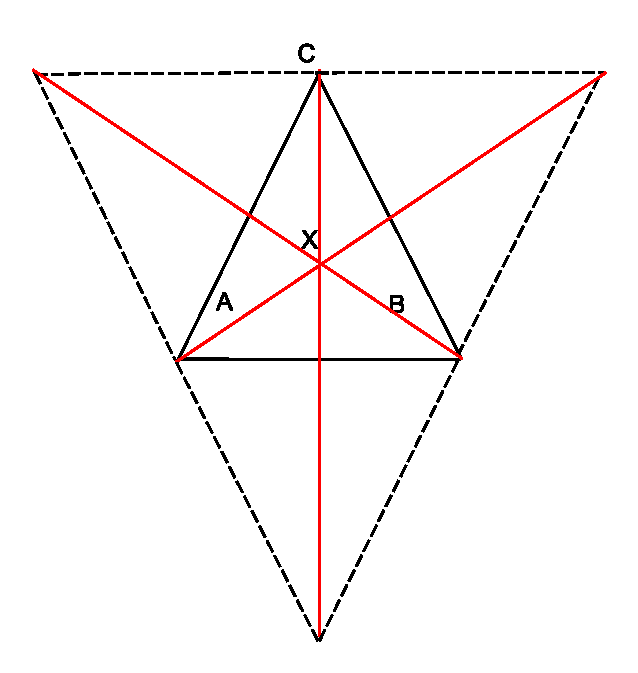
\includegraphics[width=0.7\textwidth]{fig_fermat}
    \caption{Graphical representation of the Fermat-Torricelli problem}
    \label{fig:fermat_problem}
\end{figure}


In this paper, this point was used to represent the center of the platform, that is to say point $p$ of equation~\ref{eq:p}.

In order to find this point an algebraic approach was used.
This approach is widely explained in~\cite{Palacios-Velez2015}, and it finds the $(x,y)$ coordinates of the point using the following equations:

\begin{equation}
    \label{eq:fermat_x}
    xFermat = \frac{xb(\sqrt{3}xc + yc)(xb + xc + \sqrt{3} yc)}{2\sqrt{3}(xb^2 - xb xc + xc^2 + yc^2 + \sqrt{3} xb yc)}
\end{equation}

\begin{equation}
    \label{eq:fermat_y}
    yFermat = \frac{xb(\sqrt{3}xc + yc)(\sqrt{3}(xb - xc) + yc)}{2\sqrt{3}(xb^2 - xb xc + xc^2 + yc^2 + \sqrt{3} xb yc)}
\end{equation}

where $xa, xb, xc$ represent the $x$ components of the vertices $A,B,C$ respectively, and $yc$ represents the $y$ component of the vertex $C$.

After obtaining the coordinates of the Fermat-Torricelli point on a 2-dimensional plane defined for this very purpose, the Fermat point was transformed into a 3-dimensional point which is referenced to the origin of the mechanism; the center of the base.

To transform the 2-dimensional point obtained into our 3-dimensional original plane, a cross product was performed between the $xFermat$ coordinate and the vector $\mathbf{q}_{21}$, which is the unit vector from the spherical joint 1 to the spherical joint 2.
This vectors $\mathbf{q}_{21}$ and $\mathbf{q}_{31}$ are denoted as follows:

$$ \mathbf{q}_{21} =
\begin{bmatrix}
-a+d \cose \theta_1 + \frac{1}{2}(-a +d \cose \theta_2) \\
-\frac{1}{2}\sqrt{3}(a -d \cose \theta_2) \\
-d \sen \theta_1 + d \sen \theta_2
\end{bmatrix}$$

$$ \mathbf{q}_{31} = \begin{bmatrix}
-a+d \cose \theta_1 + \frac{1}{2}(-a +d \cose \theta_3) \\
-\frac{1}{2}\sqrt{3}(a -d \cose \theta_3) \\
-d \sen \theta_1 + d \sen \theta_3
\end{bmatrix}
$$

The $xFvector$ shows how to find the vector for the $x$ coordinate in the 3-dimensional space.

\begin{equation}
    \label{eq:xFvector}
    xFvector = xFermat \times \mathbf{q}_21
\end{equation}

To obtain the $y$ component it's necessary to find a perpendicular vector to $\mathbf{q}_{21}$.
The normalized cross product of vector $\mathbf{q}_{21}$ and $\mathbf{q}_{31}$ results into a normal vector to the platform which we call $normal$.

%q31 -> {-a+dCos[θ_1]+1/2(-a+dCos[θ_3]),-1/2 √3(a-dCos[θ_3]),-dSin[θ_1]+dSin[θ_3]}

If another cross product is performed with the vector $\mathbf{q}_{21}$, a perpendicular vector to $\mathbf{q}_{21}$ is obtained. We call this vector $perp$.

%q21 -> {-a+dCos[θ_1]+1/2(-a+dCos[θ_2]),1/2 √3(a-dCos[θ_2]),-dSin[θ_1]+dSin[θ_2]}

Now a cross product between $yFermat$ coordinate and the vector obtained results into a vector from the spherical joint 1 which is perpendicular to vector $q_{21}$:

\begin{equation}
    \label{eq:yFVector}
    yFvector = yFermat \times perp
\end{equation}
%yFvector =

The sum of both vectors result into a vector from the spherical joint 1 and pointing to the center of the platform.
This is equal to vector $b$, but pointing in the opposite direction.
The final position of the center of the platform can be obtained by the sum of the vectors obtained, the $a$ and $d$ vectors of leg 1.
It's important to notice that these vectors are represented for leg 1.
If the vectors obtained with the Torricelli-Fermat analysis are summed
to the $a$ and $d$ vectors of another leg, the point obtained will not be the center of the platform but another point in space instead.

\begin{equation}
    \label{eq:p_Fermat}
    p = a_1 + d_1 + xFvector + yFvector
\end{equation}

Knowing the final position of the platform and the magnitude of the active joints, it is simple to obtain the orientation of the platform.
The equations for $\alpha, \beta$ and $\gamma$ can be obtained from Equation~\ref{eq:d}.

Considering that $\mathbf{b}_i$ can be seen as $\mathbf{b}_i =\{b_x, b_y, b_z\}$ the orientation of the platform is determined by

\begin{equation}
    \label{eq:beta}
    \beta = \arcsin \left( -\mathbf{b}_z \right)
\end{equation}

A normal vector $\mathbf{n}$ was obtained for the platform. The cross product $\mathbf{w}$ is then denoted as $\mathbf{w} = \mathbf{b} \times \mathbf{n}$.

The rest of the orientation angles can then be seen as

\begin{equation}
    \label{eq:alpha}
    \alpha = \arcsin \left(\frac{\mathbf{w}_z}{\cose \beta} \right)
\end{equation}

and

\begin{equation}
    \label{eq:gamma}
    \gamma = \arcsin \left( \frac{\mathbf{b}_y}{\cose \beta} \right)
\end{equation}

\section{Inverse Kinematic Analysis}
\label{sec:inverse}

The inverse position problem refers to obtaining the angles of the active joints required to obtain a certain specific position and orientation of the platform.
A 9-equation system is defined when Equation~\ref{eq:p} is written for each limb, substituting the values $\psi_1 = \chi_1 = 0\degree, \psi_2 = \chi_2 = 120\degree$ and $\psi_3 = \chi_3 = 240\degree$.

The equation system is defined for the unknown variables $\mathbf{b}_1, \mathbf{b}_2, \mathbf{b}_3, \theta_1, \theta_2, \theta_3, \mathbf{p}_x, \mathbf{p}_y$ and $\gamma$.
The software Wolfram Mathematica 11.1 was used to try and find the solution of the equation system, considering the known parameters $a, d$ and the 3 degrees of freedom determined by position $\mathbf{p}_z$ and orientation $\alpha$ and $\beta$.

However, after several days, the software raised an \texttt{OutOfMemory} exception. Additional details are included in Section~\ref{sec:problems}.

To reduce the complexity of the solution, three additional equations were used to limit the range of the three $\theta$ angles, from $0\deg$ to $180\deg$ each.
Nevertheless, this treatment was of no use since many days later the solver ran out of memory as before.

In order to reduce the amount of unknown variables in the equation system, de la Torre and Rodríguez-Leal proposed a geometric approach to find the position and orientation of the platform~\cite{delaTorre2016}.

This approach was adopted since both mechanisms (3-RSP and 3-CRC) are affected by the same parasitic movements.
Using this method, two components of the platform were obtained: $p_x$ and $p_y$, as well as the critical rotation of the platform, $\gamma$.
The resulting equations are the following:

\begin{equation}
    \label{eq:px_3crc}
    p_x = \frac{a_1 (-1 + \cose \beta \sec \alpha)(1 + \cose \beta \sec \alpha)^2 - a_1 (1 + 3 \cose \beta \sec \alpha) \sen \beta \tan^2 \alpha}{2(\cose \beta + \sec \alpha)^2}    
\end{equation}

\begin{equation}
    p_y = \frac{a_1 \sen \beta((3 \cose \alpha - \cose \beta)(\cose \alpha + \cose \beta) + 3 \sen^2 \alpha \sen^2 \beta) \tan \alpha}{2(1 + \cose \alpha \cose \beta)^2}
\end{equation}

\begin{equation}
    \gamma = \arctan \left( \frac{\sen \alpha \sen \beta}{\cose \alpha + \cose \beta} \right)
\end{equation}

This approach reduced the amount of unknown variables to six down from nine.
However, the solver ran out of memory even quicker: just 30 minutes after starting.

To try to solve the problem quicker in order to reduce the amount of memory used, a parallel approach was developed.
The solver was then executed using 4 Mathematica Kernels, which ended up running out of memory 10 minutes after starting.

Memory management procedures were implemented, as well as limiting the amount of processors used by each kernel with no luck.
Finally, memory sharing and memory limit per variable was implemented for each kernel.
The solver managed to stabilize at 70\% of memory usage in a 10-GB RAM environment, and was left for nearly twelve days to obtain the solution.
Unfortunately, no solution has been found as the date of this report.
Additional computer and solver details are described in Section~\ref{sec:problems}

\section{Mobility Analysis}
\label{sec:mobility}

An important question regarding parallel mechanisms is to determine their mobility.
The mobility represents the number of inner degrees of freedom of a mechanism.
The mobility analysis of this robot was performed through the use of screw theory.

The motion-screw set is composed of five independent joint screws $\$_{ij}$.
Screw $\$_{i1}$ is a rotational screw corresponding to the revolute joint.
For simplification purposes, the spherical joint can be seen as three independent rotational screws: $\$_{i2}, \$_{i3}, \$_{i4}$, where the joint axes are considered to be invariantly parallel to the $X$, $Y$ and $Z$ axes, respectively.
Finally, screw $\$_{i5}$ is a translational screw corresponding to the prismatic joint.
The complete screw system can be seen as:

\begin{equation}
    \label{eq:screw-initial-sys}
    \begin{bmatrix}
        \$_{i1} \\
        \$_{i2} \\
        \$_{i3} \\
        \$_{i4} \\
        \$_{i5} \\
    \end{bmatrix}
    =
    \begin{bmatrix}
        -\sen \psi_i & \cose \psi_i & 0 & 0 & 0 & a \\
        1 & 0 & 0 & 0 & d\sen \theta_i & -a + (d \cose \theta_i)\sen \psi_i \\
        0 & 1 & 0 & -d \sen \theta_i & 0 & (a - d \cose \theta_i)\cose \psi_i \\
        0 & 0 & 1 & (a -d \cose \theta_i)\sen \psi_i & (-a + d \cose \theta_i)\cose \psi_i & 0 \\
        0 & 0 & 0 & U_x \cose \chi_i  + V_x \sen \chi_i & U_y \cose \chi_i + V_y \sen \chi_i & U_z \cose \chi_i + V_z \sen chi_i
    \end{bmatrix}
\end{equation}

where $U_j, V_j$ represent the $j$-th component of the columns $U, V$ in Equation~\ref{eq:RM_matrix}, and the unit vectors for each screw are:

\begin{equation}
    \label{eq:screw_init_sys_units}
    \begin{bmatrix}
     -\sen \psi _i & \cose \psi _i & 0 \\
     1 & 0 & 0 \\
     0 & 1 & 0 \\
     0 & 0 & 1 \\
     U_x \cose \chi _i + V_x \sen \chi _i& U_y \cose \chi _i +V_y \sen \chi _i & U_z \cose \chi _i + V_z \sen \chi _i \\
    \end{bmatrix}
\end{equation}

To analyze the mobility of the robot, the method proposed by Dai is used in this paper~\cite{Rodriguez-Leal10}, which consists of:

\begin{enumerate}
    \item Obtain the branch motion-screw system for each limb
    \item Computation of the branch constraint-screw system for each limb that is reciprocal to the motion-screw system. These systems describe the motion and constraint of the moving platform to the base, respectively.
    \item Obtain the platform constraint-screw system ($S_c$) that is formed by the combination of the independent basis of the motion system in previous point.
    \item Calculation of the reciprocal of $S_c$, which results in the platform motion-screw system $S_f$.
\end{enumerate}

The branch motion-screw system matrix is composed of the five screws of Equation~\ref{eq:screw-initial-sys}.

The branch constraint-screw system matrix for every limb is obtained by computing the reciprocal of the motion-screw system in~\ref{eq:screw-initial-sys}:

\begin{equation}
    \label{eq:constraint-screw1}
    \frac{\cose \chi _i U_z+\sen \chi _i V_z \tan \psi _i-\cot \theta _i \sec \psi _i \cose \chi _i U_y+\sen \chi _i V_y}{\cose \chi _i U_y+\sen \chi _i V_y-\cose \chi _i U_x+\sen \chi _i V_x \tan \psi _i}
\end{equation}

\begin{equation}
    \label{eq:constraint-screw2}
    \frac{\cose \psi _i \cose \chi _i U_z+\sen \chi _i V_z-\cot \theta _i \cose \chi _i U_x+\sen \chi _i V_x}{\sen \psi _i \cose \chi _i U_x+\sen \chi _i V_x-\cose \psi _i \cose \chi _i U_y+\sen \chi _i V_y}
\end{equation}

\begin{equation}
    \label{eq:constraint-screw3}
    1
\end{equation}

\begin{equation}
    \label{eq:constraint-screw4}
    \resizebox{0.95\hsize}{!}{%
        $\frac{a+d \cose \theta _i \cose \chi _i U_x+\sen \chi _i V_x+d \cose \theta _i-a \cose (2 \psi _i) \cose \chi _i U_x+\sen \chi _i V_x+d \cose \theta _i-a \sen (2 \psi _i) \cose \chi _i U_y+\sen \chi _i V_y-2 d \cose \psi _i \sen \theta _i \cose \chi _i U_z+\sen \chi _i V_z}{2 \sen \psi _i \cose \chi _i U_x+\sen \chi _i V_x-2 \cose \psi _i \cose \chi _i U_y+\sen \chi _i V_y}$%
    }
\end{equation}

\begin{equation}
    \label{eq:constraint-screw5}
    \resizebox{0.95\hsize}{!}{%
    $\frac{a-d \cose \theta _i \cose \chi _i \sen \psi _i U_x+\sen \chi _i a-d \cose \theta _i \sen \psi _i V_x-a \sec \psi _i V_y+a-d \cose \theta _i \sen \chi _i \sen \psi _i V_y+d \sen \theta _i \cose \chi _i U_z+\sen \chi _i V_z \tan \psi _i-\cose \chi _i U_y a \cose \psi _i+d \cose \theta _i \sen \psi _i \tan \psi _i}{\cose \chi _i U_y+\sen \chi _i V_y-\cose \chi _i U_x+\sen \chi _i V_x \tan \psi _i}$%
    }
\end{equation}

\begin{equation}
    \label{eq:constraint-screw6}
    -\frac{a-d \cose \theta _i \cose \chi _i \cose \psi _i \cot \theta _i U_x+\cose \chi _i \cot \theta _i \sen \psi _i U_y-\cose \chi _i U_z+\sen \chi _i \cot \theta _i \cose \psi _i V_x+\sen \psi _i V_y-V_z}{\sen \psi _i \cose \chi _i U_x+\sen \chi _i V_x-\cose \psi _i \cose \chi _i U_y+\sen \chi _i V_y}
\end{equation}

Substituting for each leg, we get

\begin{equation}
    \label{eq:rb1}
    \$_{rb1} =
    \begin{bmatrix}
     -\cot\theta _1 \\
     \frac{\cot\theta _1 U_x-U_z}{U_y} \\
     1 \\
     \frac{d\sen\theta _1 U_z-\cose\theta _1 U_x}{U_y} \\
     -a \\
     \frac{(a-d \cose\theta _1)\cot\theta _1 U_x-U_z}{U_y}
    \end{bmatrix}
\end{equation}

\spacepls

\begin{equation}
    \label{eq:rb2}
    \$_{rb2} =
    \begin{bmatrix}
     \frac{-\sqrt{3} U_z+2 \cot \left(\theta _2\right) \left(U_y-\sqrt{3} V_y\right)+3 V_z}{\sqrt{3} U_x+U_y-3 V_x-\sqrt{3} V_y} \\
     \frac{-2 \cot \left(\theta _2\right) U_x-U_z+\sqrt{3} \left(2 \cot \left(\theta _2\right) V_x+V_z\right)}{\sqrt{3} U_x+U_y-3 V_x-\sqrt{3} V_y} \\
     1 \\
     \frac{3 a+d \cose \left(\theta _2\right)+\frac{2 d \sen \left(\theta _2\right) \left(\sqrt{3} U_z-3 V_z\right)-4 d \cose \left(\theta _2\right) \left(U_y-\sqrt{3} V_y\right)}{\sqrt{3} U_x+U_y-3 V_x-\sqrt{3} V_y}}{2 \sqrt{3}} \\
     \frac{1}{2} \left(a-d \cose \left(\theta _2\right)\right)+\frac{2 d \cose \left(\theta _2\right) \left(U_y-\sqrt{3} V_y\right)+d \sen \left(\theta _2\right) \left(3 V_z-\sqrt{3} U_z\right)}{\sqrt{3} U_x+U_y-3 V_x-\sqrt{3} V_y} \\
     \frac{\left(a-d \cose \left(\theta _2\right)\right) \left(\cot \left(\theta _2\right) \left(U_x-\sqrt{3} U_y-\sqrt{3} V_x+3 V_y\right)+2 \left(U_z-\sqrt{3} V_z\right)\right)}{\sqrt{3} U_x+U_y-3 V_x-\sqrt{3} V_y} \\
    \end{bmatrix}
\end{equation}

\spacepls

\begin{equation}
    \label{eq:rb3}
    \$_{rb3} =
    \begin{bmatrix}
     \frac{\sqrt{3} U_z+2 \cot \theta _3 U_y+\sqrt{3} V_y+3 V_z}{-\sqrt{3} U_x+U_y-3 V_x+\sqrt{3} V_y} \\
     \frac{2 \cot \theta _3 U_x+U_z+\sqrt{3} 2 \cot \theta _3 V_x+V_z}{\sqrt{3} U_x-U_y+3 V_x-\sqrt{3} V_y} \\
     1 \\
     \frac{-3 a-d \cose \theta _3+\frac{-4 d \cose \theta _3 U_y+\sqrt{3} V_y-2 d \sen \theta _3 \sqrt{3} U_z+3 V_z}{\sqrt{3} U_x-U_y+3 V_x-\sqrt{3} V_y}}{2 \sqrt{3}} \\
     \frac{1}{2} a-d \cose \theta _3+\frac{d 2 \cose \theta _3 U_y+\sqrt{3} V_y+\sen \theta _3 \sqrt{3} U_z+3 V_z}{-\sqrt{3} U_x+U_y-3 V_x+\sqrt{3} V_y} \\
     -\frac{a-d \cose \theta _3 \cot \theta _3 U_x+\sqrt{3} U_y+\sqrt{3} V_x+3 V_y+2 U_z+\sqrt{3} V_z}{\sqrt{3} U_x-U_y+3 V_x-\sqrt{3} V_y}
    \end{bmatrix}
\end{equation}

The motion-screw system is obtained via analyzing the reciprocal of the constraint-screw system: an $\$r = \{\$_{rb1}, \$_{rb2}, \$_{rb3}\}$ was obtained using Equations~\ref{eq:rb1}, \ref{eq:rb2} and \ref{eq:rb3}.
The reciprocal of $\$r$ was labeled as $\$_{f}$, containing $\$f_1, \$f_2$ and $\$f_3$.
$\$_f$ represents the mobility of the platform.

\section{Velocity Analysis}
\label{sec:velocity}

Mathematically, the forward kinematic equations define a function between the space of Cartesian positions and orientations and the space of joint positions.
The relation of velocities for these equations are then determined in the velocity analysis, also know as instantaneous kinematic analysis, through the Jacobian matrix of this function.
The Jacobian matrix can be determined by applying the theory of reciprocal screws and by using a method proposed by Joshi and Tsai~\cite{Joshi02}.

The first step is to perform the calculation of the Jacobian of constraints $J_c$, which is composed by those unit screws that are reciprocal to all the joint screws of the $i$-th limb:

\begin{equation}
\label{eq:Jc}
    J_c =\left\{\frac{P}{\rho}, \frac{Q}{\rho}, \frac{R}{\rho} ; \frac{L}{\rho}, \frac{M}{\rho}, \frac{N}{\rho}\right\}
\end{equation}

where $\rho$ is the magnitude of the vector.

As seen in previous sections, each leg posses one reciprocal screw, which is the general reciprocal screw $\$_{rbi}$.
By definition a unit vector is a vector with length 1.
To calculate the unit vector of any vector it’s only necessary to divide each component by the vectors norm.
Calculating the unit vector for $\$_{rbi}$, results into dividing each element by a factor labeled as $\rho$ (See Mathematica files).

The Jacobian of constraints $Jc$ is obtained by applying the orthogonal product of the reciprocal unit-screw for each limb and by rearranging these results in matrix form.

The following step is to compute the Jacobian of actuation $J_a$.
This step is done by \textit{locking} the actuated joint of each limb,
which in this case is the revolute joint.
This will generate the same $\$_{rbi}$ screws and additional reciprocal screw that will be calculated for each leg.
The Jacobian of actuation is denoted as:

\begin{equation}
\label{eq:Ja}
\resizebox{0.94\textwidth}{!}{%
$J_a =
\begin{bmatrix}
 0 & -a+d \cose \left(\theta _1\right)-\frac{d \sen \left(\theta _1\right) U_z}{U_x} & 0 & -\frac{U_z}{U_x} & 0 & 1 \\
 \frac{1}{2} \sqrt{3} \left(a-d \cose \left(\theta _2\right)\right) & \frac{1}{2} \left(a-d \cose \left(\theta _2\right)+\frac{2 d \sen \left(\theta _2\right) \left(\sqrt{3} V_z-U_z\right)}{U_x-\sqrt{3} V_x}\right) & \frac{\left(a-d \cose \left(\theta _2\right)\right) \left(\sqrt{3} U_z-3 V_z\right)}{2 \left(U_x-\sqrt{3} V_x\right)} & \frac{\sqrt{3} V_z-U_z}{U_x-\sqrt{3} V_x} & 0 & 1 \\
 -\frac{1}{2} \sqrt{3} \left(a-d \cose \left(\theta _3\right)\right) & \frac{1}{2} \left(a-d \cose \left(\theta _3\right)-\frac{2 d \sen \left(\theta _3\right) \left(U_z+\sqrt{3} V_z\right)}{U_x+\sqrt{3} V_x}\right) & -\frac{\left(a-d \cose \left(\theta _3\right)\right) \left(\sqrt{3} U_z+3 V_z\right)}{2 \left(U_x+\sqrt{3} V_x\right)} & -\frac{U_z+\sqrt{3} V_z}{U_x+\sqrt{3} V_x} & 0 & 1
\end{bmatrix}$%
}
\end{equation}

The final Jacobian matrix is then composed of both the Jacobian of actuation and  the Jacobian of constraints joined.
It is a $6 \times 6$ matrix.

\begin{equation}
    \label{eq:final_jacobian}
    \resizebox{0.94\textwidth}{!}{%
    $J =
        \begin{bmatrix}
            0 & -a+d \cose \left(\theta _1\right)-\frac{d \sen \left(\theta _1\right) U_z}{U_x} & 0 & -\frac{U_z}{U_x} & 0 & 1 \\
            \frac{1}{2} \sqrt{3} \left(a-d \cose \left(\theta _2\right)\right) & \frac{1}{2} \left(a-d \cose \left(\theta _2\right)+\frac{2 d \sen \left(\theta _2\right) \left(\sqrt{3} V_z-U_z\right)}{U_x-\sqrt{3} V_x}\right) & \frac{\left(a-d \cose \left(\theta _2\right)\right) \left(\sqrt{3} U_z-3 V_z\right)}{2 \left(U_x-\sqrt{3} V_x\right)} & \frac{\sqrt{3} V_z-U_z}{U_x-\sqrt{3} V_x} & 0 & 1 \\
            -\frac{1}{2} \sqrt{3} \left(a-d \cose \left(\theta _3\right)\right) & \frac{1}{2} \left(a-d \cose \left(\theta _3\right)-\frac{2 d \sen \left(\theta _3\right) \left(U_z+\sqrt{3} V_z\right)}{U_x+\sqrt{3} V_x}\right) & -\frac{\left(a-d \cose \left(\theta _3\right)\right) \left(\sqrt{3} U_z+3 V_z\right)}{2 \left(U_x+\sqrt{3} V_x\right)} & -\frac{U_z+\sqrt{3} V_z}{U_x+\sqrt{3} V_x} & 0 & 1 \\
            \frac{P_1}{\rho}& \frac{Q_1}{\rho}& \frac{R_1}{\rho} & \frac{L_1}{\rho}& \frac{M_1}{\rho}& \frac{N_1}{\rho}\ \\
            \frac{P_2}{\rho}& \frac{Q_2}{\rho}& \frac{R_2}{\rho} & \frac{L_2}{\rho}& \frac{M_2}{\rho}& \frac{N_2}{\rho}\ \\
            \frac{P_3}{\rho}& \frac{Q_3}{\rho}& \frac{R_3}{\rho} & \frac{L_3}{\rho}& \frac{M_3}{\rho}& \frac{N_3}{\rho}
    \end{bmatrix}$%
    }
\end{equation}

\section{Singularities}
\label{sec:singular}

One of the primary interests in manipulator velocity analysis is to determine the presence and location of any singular positions.
The physical implication of a singular position is that the manipulator loses one or more degrees of freedom of output motion.

A singularity occurs when the joint velocity in joint space becomes infinite.
It shows us where the continuity in joint space breaks down as related to Cartesian space.
Intuitively, this means that a singularity is a point in the workspace where the robot loses its ability to move the end effector in some direction no matter how it moves its joints.

A singularity occurs whenever the determinant of the Jacobian matrix is 0.
The associated Jacobian matrix is said to be singular if this is the case.
To find when this occurs we set

\begin{equation}
\label{eq:singular_det0}
    \text{det}(J) = 0
\end{equation}

and solve for the singularity.

\section{Static Analysis}
\label{sec:static}

The static analysis is realized to obtain the interaction of forces and torques in steady state, where no motion is performed.
The 3-RSP mechanism was divided into two sections in order to perform the analysis.
The first one consists of the link $d_i$ placed between the rotative joint and the spherical joint.
The second section corresponds to the link between the platform and the three spherical joints. Both sections and their respective free-form diagrams are shown on Fig.~\ref{fig:static}.

\begin{figure}[htbp]
\centering
\begin{subfigure}[b]{0.45\textwidth}
\includegraphics[width=1\linewidth]{static01}
\end{subfigure}
\begin{subfigure}[b]{0.45\textwidth}
\includegraphics[width=1\linewidth]{static02}
\end{subfigure}
\begin{subfigure}[b]{0.45\textwidth}
\includegraphics[width=1\linewidth]{static03}
\end{subfigure}
\begin{subfigure}[b]{0.45\textwidth}
\includegraphics[width=1\linewidth]{static04}
\end{subfigure}
\caption{3-RSP sections and free-form diagrams}
\label{fig:static}
\end{figure}

The analysis is done considering $\sum F = 0$.
$R_{ij}$ is the reaction force for each joint $j$ for leg $i$.
The reaction forces for section one and two are:

\begin{equation}
    \label{eq:reaction_for_section1}
    R_{i1} + R_{i2} + R_{i3} = R_{i4} \,\,\,\, \text{(Section 1)}
\end{equation}

\begin{equation}
    F_{s1} + F_{s2} + F_{s3} + W = 0 \,\,\,\, \text{(Section 2)}
\end{equation}

The sum of moments is then

\begin{equation}
    \label{eq:sum_of_moments_sec1}
    -M_{i1} -M_{i2} -M_{i3} + M_{i4} + d_i \times R_{i4} = 0 \,\,\,\, \text{(Section 1)}
\end{equation}

\begin{equation}
    \label{eq:sum_of_moments_sec2}
    -b_1 \times F_{s1} - b_2 \times F_{s2} -b_3 \times F_{s3} + M_{s1} + M_{s2} + M_{s3} = 0 \,\,\,\, \text{(Section 2)}
\end{equation}

Where $F_{si}$ and $M_{si}$ are

\begin{equation}
    F_{si} = R_{i1} + R_{i2} + R_{i3}
\end{equation}

\begin{equation}
    M_{si} = M_{i1} + M_{i2} + M_{i3}
\end{equation}

\section{Dynamic Analysis}
\label{sec:dynamic}

The dynamic analysis is the determination of motions mechanism as a function of time.
This function must be determined from the action of the forces to which the mechanism is subject to.
The dynamic analysis determines the relation between forces and motion: torque values for each link.

If

\begin{equation}
  \label{eq:dynamic_vi}
  v_i = J_{v_i}(q)\dot{q}
\end{equation}

and 

\begin{equation}
    \label{eq:dynamiv_omegai}
    \omega_i = J_{\omega_i}(q)\dot{q}
\end{equation}

then the overall kinetic energy of the manipulator is

\begin{equation}
    \label{eq:kinetic_energy}
    K = \frac{1}{2}\dot{q}^T \sum_{i=1}^n (m_i J_{v_i} q^T J_{v_i}(q) + J_{\omega_i} q^T R_i (q) I_i R_i q^T J_{\omega_i} (q)) \dot{q}
\end{equation}

where $m_i$ is the mass of link $i$,
Assuming that the mass of the mechanism is concentrated at its center of mass, then the total potential energy is

\begin{equation}
    \label{eq:potential_energy}
    P = \sum_{i=1}^n P_i = \sum_{i=1}^n g^T r_{ci} m_i
\end{equation}

Where $g$ is the vector of gravity and $r_{ci}$ are the coordinates of the center of mass of link $i$.

\section{Motion Study}
\label{sec:motion_study}

The motion study of the mechanism was developed in Solidworks, using the assembled model to determine the physical movements under the effect of a rotary motor situated on the platform and rotation through the $x$-axis,
and a second rotary motor rotating through the $y$-axis.
This is not the position of the actuators in the physical design,
since they are located at the rotative joints,
but in terms of simulation this is used in order to predict the movement available on the platform.
The analysis of the components is shown in Fig.~\ref{fig:motion}.

\begin{figure}[htbp]
    \centering
    \begin{subfigure}[b]{0.65\textwidth}
        \includegraphics[width=\linewidth]{AlphaBetaGamma_sw}
        \caption{}
    \end{subfigure}
    \begin{subfigure}[b]{0.65\textwidth}
        \includegraphics[width=\linewidth]{bi_sw}
        \caption{}
    \end{subfigure}
    \begin{subfigure}[b]{0.65\textwidth}
        \includegraphics[width=\linewidth]{PxPyPz_sw}
        \caption{}
    \end{subfigure}
    \begin{subfigure}[b]{0.65\textwidth}
        \includegraphics[width=\linewidth]{Theta_sw}
        \caption{}
    \end{subfigure}
    \caption{Motion study of the 3-RSP.
    (a) The analysis for the $\alpha, \beta$ and $\gamma$ orientation angles.
    (b) Analysis of the lengths of $b_i$ (prismatic joints).
    (c) Analysis of the position of the center of the platform ($p_x, p_y, p_z$).
    (d) Analysis of the $\theta$ angles (revolute joints).}
    \label{fig:motion}
\end{figure}

The $\alpha, \beta, \gamma$ (Fig.~\ref{fig:motion} (a)) chart shows the projection angles of the platform when the motors actuate a rotation of 5\textdegree to one direction, and return; and to the other direction, and return.
It was not expected to have motion on the $\gamma$ angle, however in the chart appears a movement of about 0.013\textdegree which indicates a parasitic motion.

On Fig.~\ref{fig:motion} (b), the displacement of the three prismatic joint –the length of $\textbf{b}_i$– is presented.
It was necessary to adjust the motion study to a very soft movement, since some of the assembled joints were corrupted with a higher motion.
The prismatic motion in this chart shows that one has a major displacement while the other two react to the first one.

The position of the platform $\mathbf{p}_x, \mathbf{p}_y, \mathbf{p}_z$ is shown on Fig.~\ref{fig:motion}.
This plot shows movement barely noticeable.
$\mathbf{p}_x$ and $\mathbf{p}_y$ are only parasitic motions, and the charts shows no value for them.
$\mathbf{p}_z$ has a small displacement of 1mm.

The final chart, which is labeled as (d) in Fig.~\ref{fig:motion} shows the angle position of the $\theta$ angles for each rotative joint.
These are the joints which are actuated, but for simulation purposes they are only following the physical displacement of the rotary motors actuating under the platform.

\section{Building a prototype}
\label{sec:prototype}

A prototype was built using light and simple materials to put the motion study to the test.
All parts of the prototype were made of aluminum and tin, so that it can have fluid mobility.
These materials are also easier to move using servo motors instead of stepper motors, which would be hard to manipulate and could get somewhat expensive to get.

An Arduino board has been used to store and run the program.
The software was programmed in both Java and Arduino code to be easy to interact with, and sent to the device through the serial port.

The code can be found along the rest of the files for the project.

\begin{figure}[htbp]
    \centering
    \begin{subfigure}[b]{0.4\textwidth}
        \includegraphics[width=\linewidth]{photo01}
    \end{subfigure}
    \begin{subfigure}[b]{0.4\textwidth}
        \includegraphics[width=\linewidth]{photo02}
    \end{subfigure}
    \begin{subfigure}[b]{0.4\textwidth}
        \includegraphics[width=\linewidth]{photo03}
    \end{subfigure}
    \begin{subfigure}[b]{0.4\textwidth}
        \includegraphics[width=\linewidth]{photo04}
    \end{subfigure}
    \caption{Photos of the 3-RSP mechanism}
    \label{fig:prototype}
\end{figure}

\section{Problems found}
\label{sec:problems}

Many problems and roadblocks were encountered through the analysis process of the mechanism.
Some of these nuisances were dealt with, while some other remained unsolved.

For example, the inverse kinematic analysis presented quite a lot of problems.
Many different setups were used to test the solver:

\begin{itemize}
    \item \texttt{Solve[expr]} method using 1 Wolfram Mathematica kernel, shared between 4 physical CPUs (i5-2500K @ 3.4GHz) and a 1GB \texttt{CacheSize}. This method ran out of memory after five days, and was using a 9-equation system (plus 3 inequalities) with 9 unknown variables.
    \item Same characteristics as before, but using \texttt{ParallelEvaluate}. This method ran out of memory after 10 minutes.
    \item Same characteristics as last method, but instead using 3 Mathematica Kernels. This method ran out of memory after 3 hours, and was using a 9-equation system (plus the 3 inequalities) with 6 unknown variables.
    \item Same method, but instead using 3 physical CPUs and \texttt{CacheSize} of 0.75GB. It was aborted at 20 minutes, as it was clear it was not a good method. In this method, we used 14 equations with no luck.
    \item The same method was applied later, using 2 Mathematica kernels and shared between 2 physical CPUs. The \texttt{CacheSize} was reduced to 0.5GB, but it was again aborted at 10 minutes as this wasn't gonna be successful.
    \item The last method applied was using \texttt{NSolve} in the $\mathbb{R}$ domain, using parallel evaluation as well but sharing the available memory between the 4 Mathematica kernels (distributed on 2 physical CPUs). \texttt{CacheSize} was maintained as 0.5GB.
    This method ran for nearly 12 days (11 days 22 hours 23 minutes 13 seconds), but was aborted since no solution was found.
\end{itemize}

The different methods applied give us some insight about the complexity of the inverse kinematic problem, as well as the whole complexity of the mechanism.

Additional roadblocks were encountered while building the prototype.
The ``theoretical'' spherical joints have a wider range of mobility than the physical ones encountered.
The weight of each part (as it was built using solid links) was somewhat heavy for the servo motors to move, so additional openings were made on the parts in order to make them hollow and weight less.

\section{Conclusions}
\label{sec:conc}

This paper presented the kinematic analysis of a 3-RSP parallel mechanism.
The range of movement of the mechanism is very limited probably because of the alignment of the rotative and prismatic movements.
According to the analysis, the mechanism presents a translation along a fixed central axis represented by $z$ in the base and platform parts of the structure.
The platform also leans, this is measured by the $\alpha$ and $\beta$angles.
Parasitic movements are also present through a rotation of the platform by the angle  $\gamma$ and translations along $x$ and $y$ axis.
The presence of parasitic movements greatly increases the complexity of the analysis.

A closed-form solution to the forward position problem is included in the paper, while the inverse solution presented a high degree of complexity leading the software to use great amounts of memory and not been able to obtain a solution.
The static force and momentum analysis is presented taking into account that all the revolute joints are positioned at 90º.
The mobility analysis showed an interesting behavior, because according to previous analysis and inspection of the physical model, the platform moves along the $Z$-axis, and rotates along the $X$ and $Y$-axes, represented by $p_x$, $\alpha$ and $\beta$, then it's possible to observe parasitic displacements on $p_x$, $p_y$ and a rotation around $Z$-axis.
But according to the platform motion-screw system, the platform has 3 degrees of freedom, the three of them are rotations about $X$, $Y$ and $Z$.
Due to these complications as well as the limitation in movement, the practicality of using this mechanism is questionable.
Research on new algorithms to solve this problem are recommended, probably some type of iterative algorithm that can approximate a numerical solution will be a good first attempt, although a general solution would be ideal.

\bibliographystyle{splncs03}
\bibliography{biblio}

\end{document}